% lista de exercícios 333 - teoria geral de sistemas

\documentclass{article}
\usepackage[a4paper,
            includeheadfoot,
            top=2cm,
            right=2cm,
            bottom=3cm,
            left=3cm]{geometry}
\usepackage[OT1]{fontenc}
\usepackage{parskip}
\usepackage{graphicx}
\usepackage{enumitem}
\usepackage{pifont}
\usepackage{tikz}
\usetikzlibrary{calc, shapes}
\usepackage{amssymb}
\usepackage{amsmath}
\usepackage{hyperref} % cria os links de referencia das equacoes

\begin{document}

\underline{\textbf{Resolução da Lista de Exercícios 3}}\par
\textbf{Sistemas de Informação}\\
\textbf{Instituto Federal do Espírito Santo}\\
Campus Serra\par
\textbf{Teoria Geral de Sistemas}\\
Prof. Dr. Rodrigo Fernandes Calhau\par
Anderson A. Fraga (20222BSI0482)\\
\texttt{aafrg@tuta.io}\\  %\texttt formats the text to a typewriter style font

Elabore os Diagramas de Fluxos (entradas e saídas):
\begin{enumerate}
    \item \textbf{Hamburgueria do Tio Paulo} (\textit{Nível 1})
    \begin{figure}[!h]
        \centering
        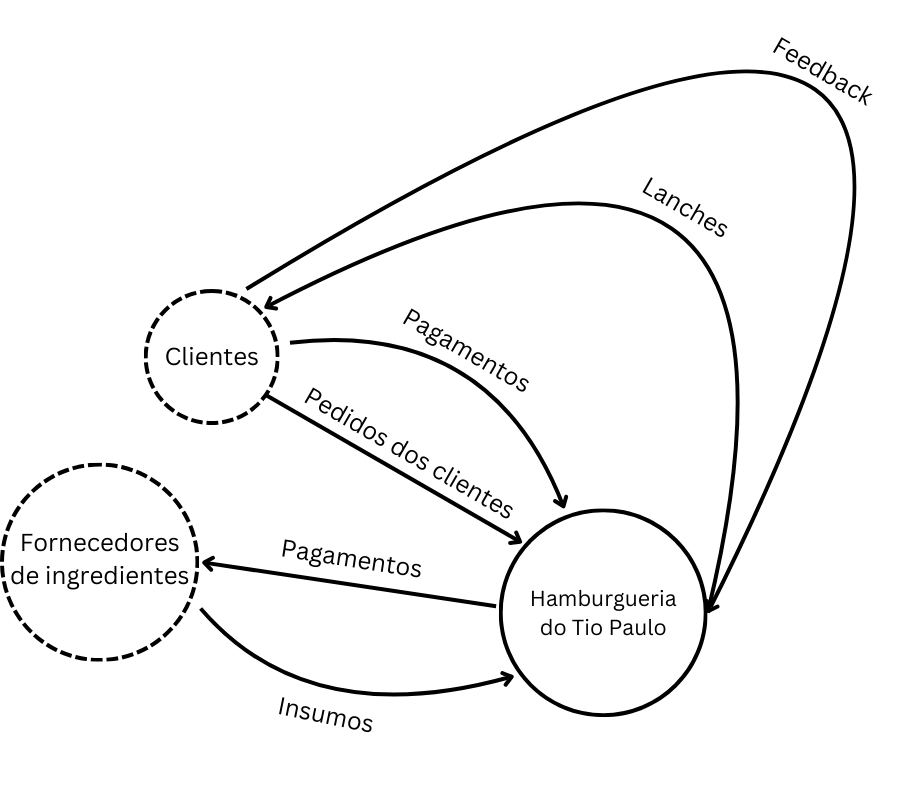
\includegraphics[width=11cm]{FIG/hamburgueria1.png}
    \end{figure}
    \pagebreak
    \item \textbf{Hamburgueria do Tio Paulo} (\textit{Nível 2})
    \begin{figure}[!h]
        \centering
        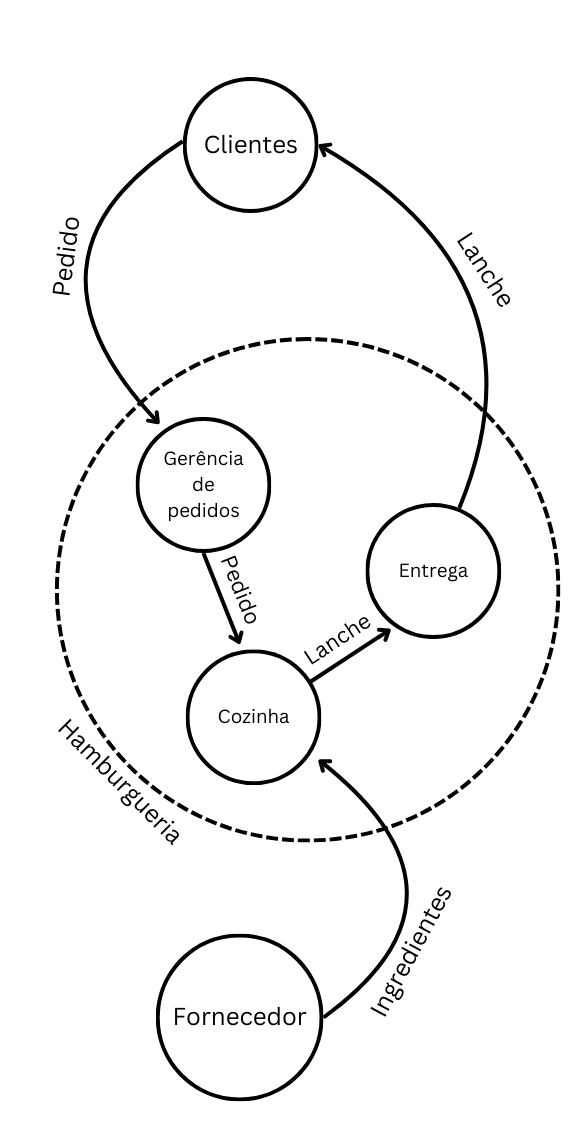
\includegraphics[width=6cm]{FIG/hamburgueria2.png}
    \end{figure}
    % \pagebreak
    \item \textbf{SoftCode} (\textit{Nível 1})
    \begin{figure}[!h]
        \centering
        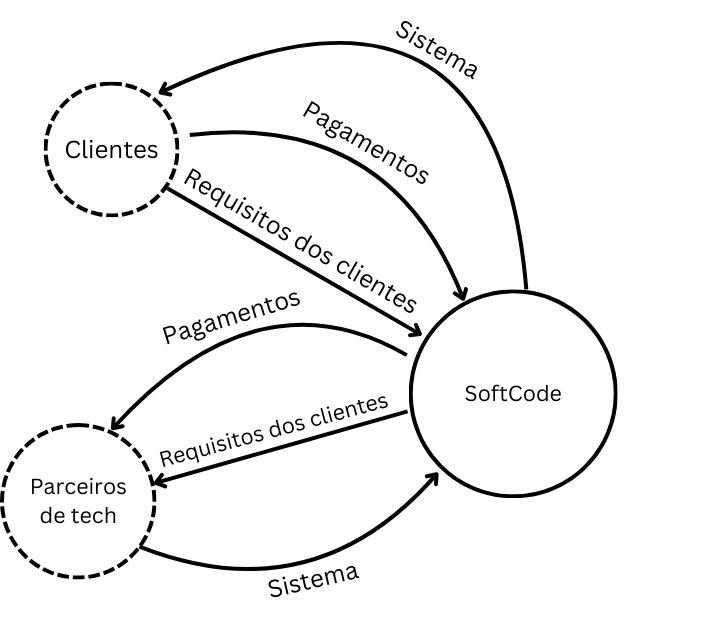
\includegraphics[width=9cm]{FIG/softcode1.png}
    \end{figure}
    \item \textbf{SoftCode} (\textit{Nível 2})
    \begin{figure}[!h]
        \centering
        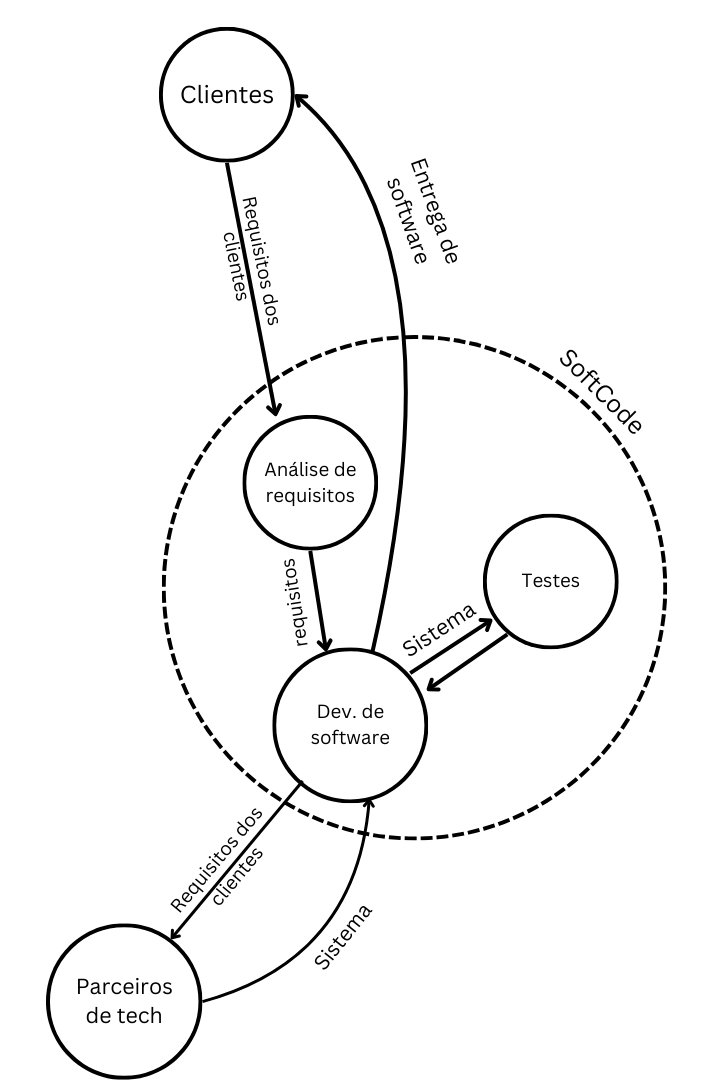
\includegraphics[width=8cm]{FIG/softcode2.png}
    \end{figure}
    \item \textbf{Clean} (\textit{Nível 1})
    \begin{figure}[!h]
        \centering
        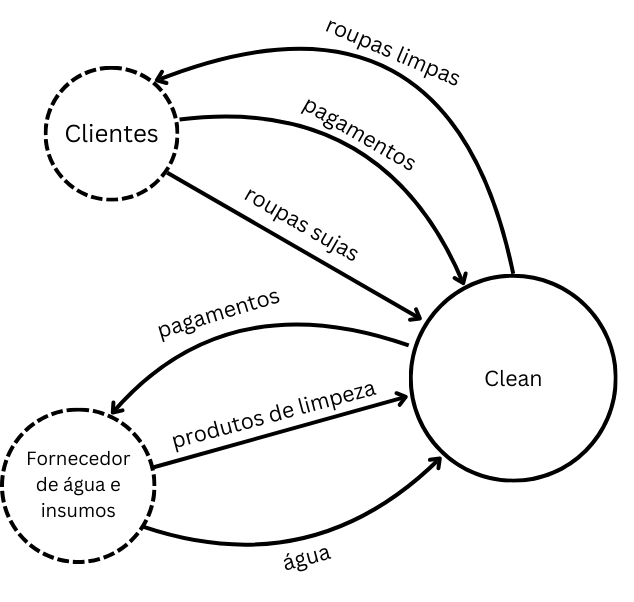
\includegraphics[width=7.5cm]{FIG/clean1.png}
    \end{figure}
    \pagebreak
    \item \textbf{Clean} (\textit{Nível 2})
    \begin{figure}[!h]
        \centering
        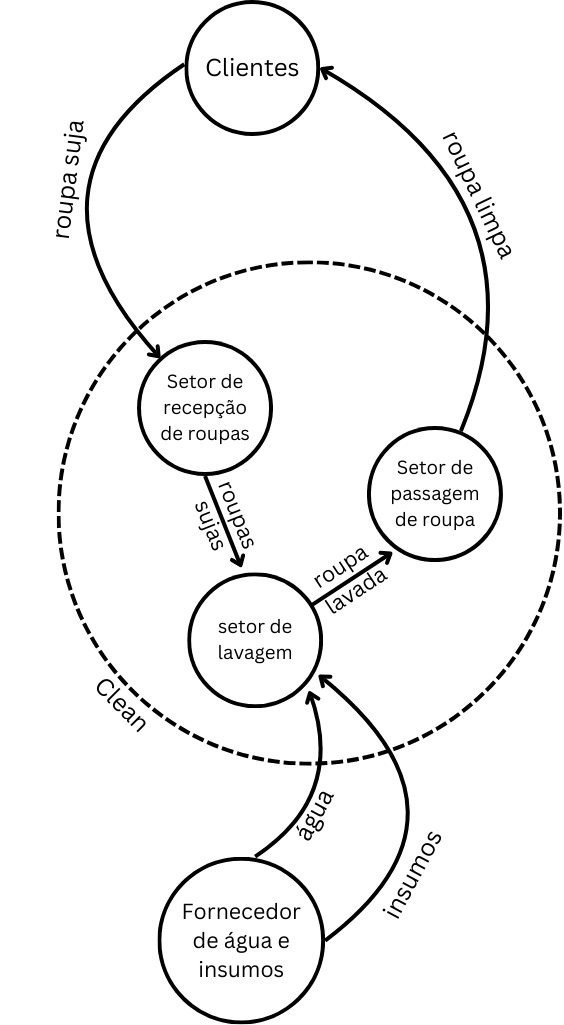
\includegraphics[width=7cm]{FIG/clean2.png}
    \end{figure}
    \item \textbf{CowHeight} (\textit{Nível 1})
    \begin{figure}[!h]
        \centering
        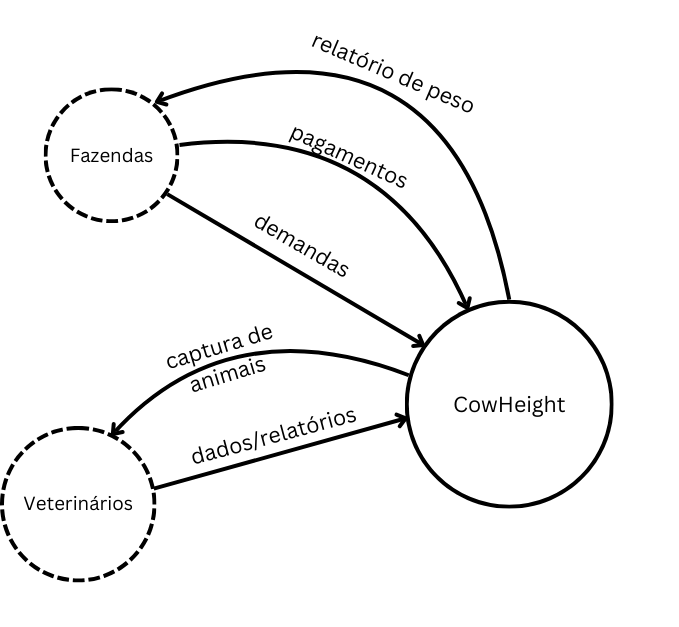
\includegraphics[width=7.7cm]{FIG/cowheight1.png}
    \end{figure}
    \item \textbf{CowHeight} (\textit{Nível 2})
    \begin{figure}[!h]
        \centering
        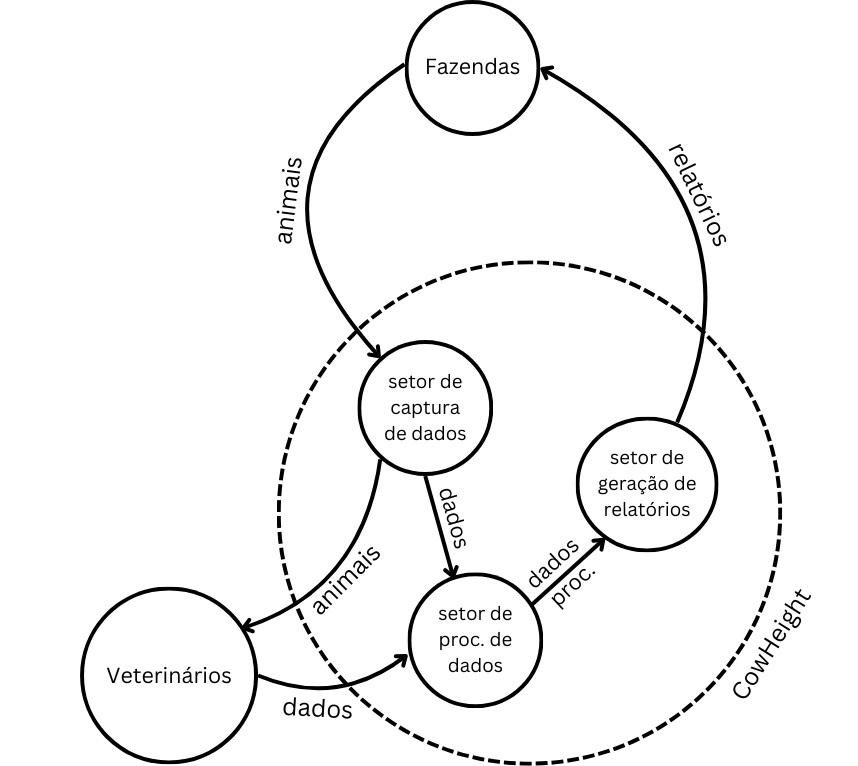
\includegraphics[width=11cm]{FIG/cowheight2.png}
    \end{figure}
    \item \textbf{Bebedouro Inteligente para Gatos} (\textit{Nível 1})
    \begin{figure}[!h]
        \centering
        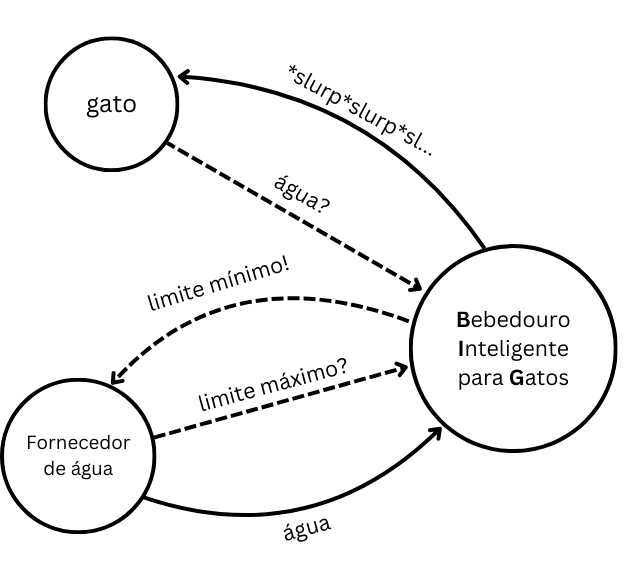
\includegraphics[width=9cm]{FIG/bebedouro1.png}
    \end{figure}
    \pagebreak
    \item \textbf{Bebedouro Inteligente para Gatos} (\textit{Nível 2})
    \begin{figure}[!h]
        \centering
        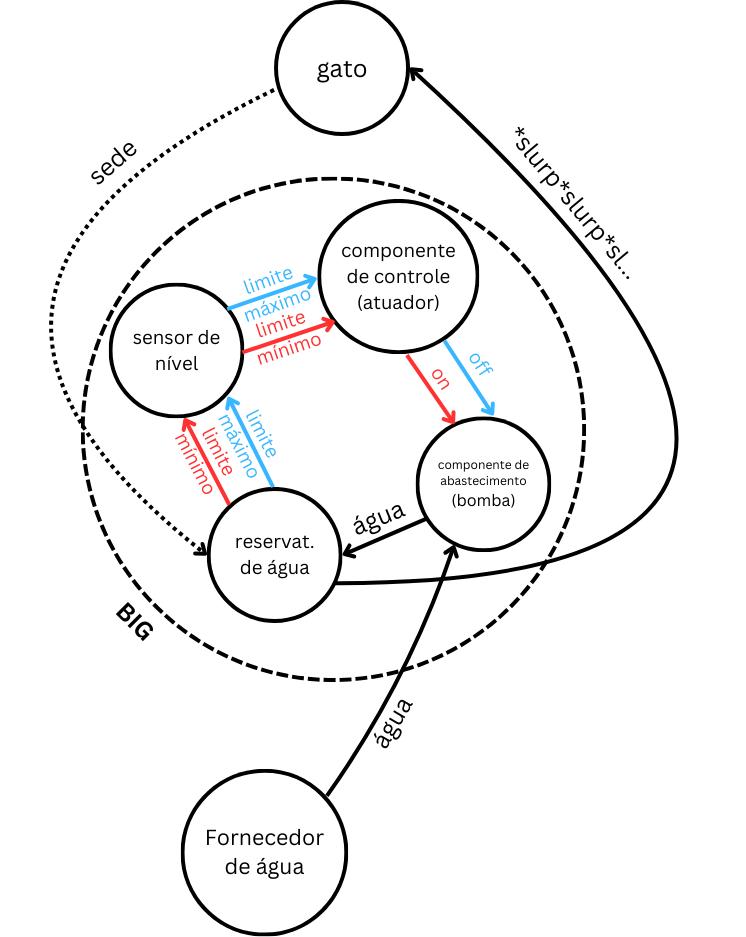
\includegraphics[width=12cm]{FIG/bebedouro3.png}
    \end{figure}
    \pagebreak
    \item \textbf{Ar-condicionado Econômico} (\textit{Nível 1})
    \begin{figure}[!h]
        \centering
        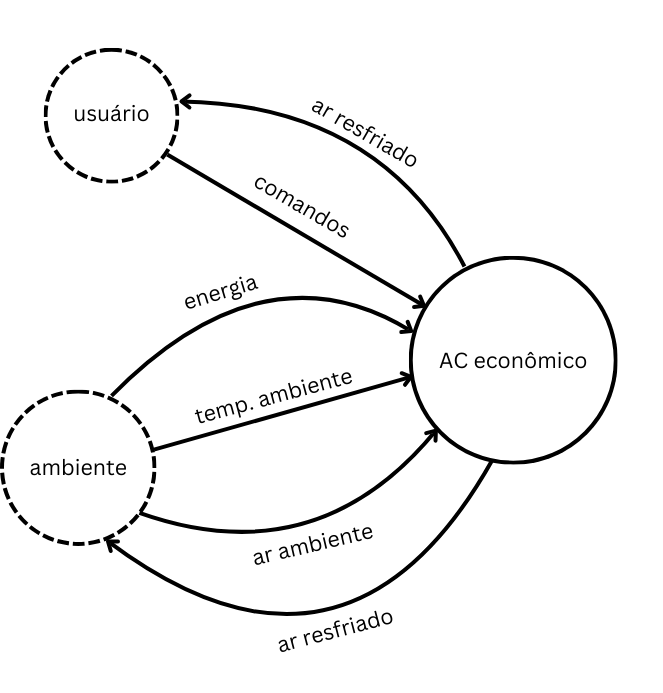
\includegraphics[width=8cm]{FIG/arcondicionado1.png}
    \end{figure}
    \item \textbf{Ar-condicionado Econômico} (\textit{Nível 2})
    \begin{figure}[!h]
        \centering
        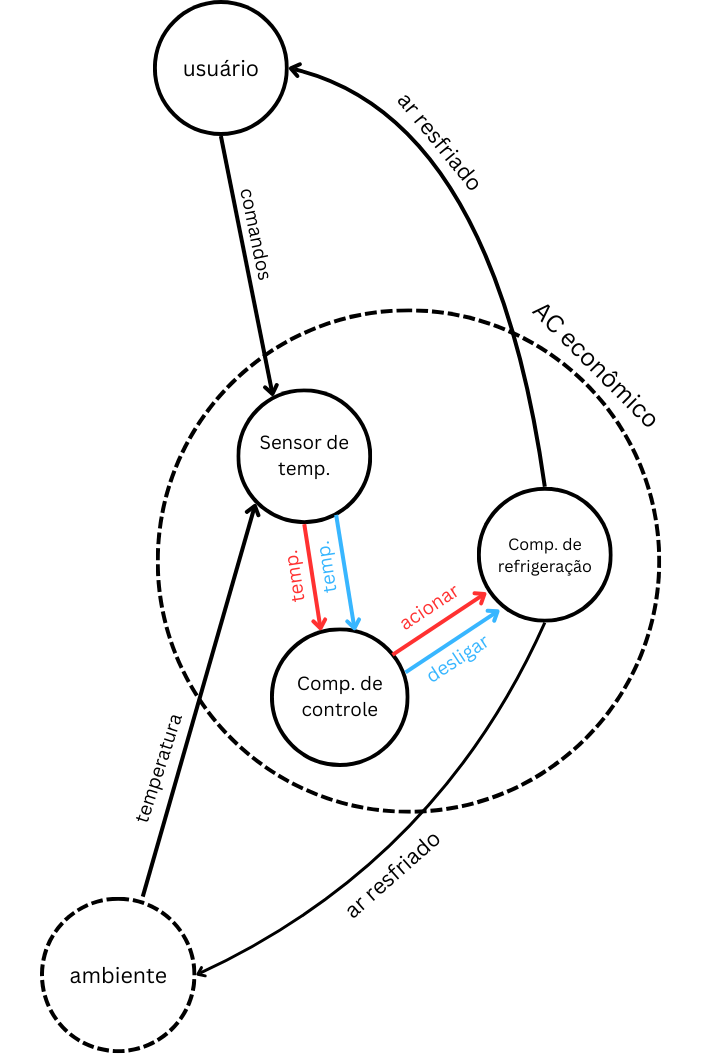
\includegraphics[width=7.7cm]{FIG/arcondicionado2.png}
    \end{figure}
\end{enumerate}\vspace{0.5cm}

\end{document}
